\begin{frame}

\frametitle{Protagonisti}

\begin{block}{Lo scanner}
\begin{itemize}
\item Scanner \emph{flat}
\item Risoluzione minima 1600 dpi non interpolati
\item Punto di illuminazione ideale diverso per ogni scanner
\end{itemize}
\end{block}
\begin{block}{Lo Shellac}
Alcune caratteristiche del disco \emph{shellac}:
\begin{itemize}
\item Diametro del disco = [8 in $\div$ 12 in]
\item Massima escursione possibile del solco $\sim$ 0.15 mm
\item Banda teorica = [30 Hz $\div$ 16000 Hz]
\item Banda reale = [500 Hz $\div$ 3500 Hz] 
\end{itemize}
\begin{center}
\emph{Solco inciso lateralemente} $\Rightarrow$ \emph{Scansione contiene forma d'onda}
\end{center}
\vspace{0.2cm}
\end{block}
\end{frame}


\begin{frame}
\frametitle{Shellac}
\begin{figure}
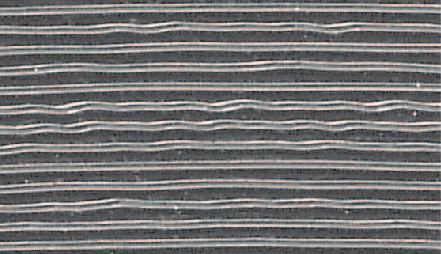
\includegraphics[width=\textwidth]{immagini/shellac-track.png}
\caption{Le tracce di uno \emph{shellac}}
\end{figure}
\end{frame}


